\chapter{Foundations}
\label{ch:Foundations}
This chapter provides an overview of the theoretical and practical foundations of \emph{Virtual Single Underlying Models} (V-SUMs), model-driven software engineering, model synchronization, and Triple Graph Grammars.

\section{Model-Driven Software Engineering}
\label{sec:Foundations:MDSE}
Model-driven software Engineering (MDSE), or sometimes referred to as model-driven software development (MDSD), is an approach to software engineering that Kramer \cite{kramer_specification_2017} describes as
\enquote{a development paradigm in which models are used in an automated way for all development tasks}.
Well-known approaches to this paradigm are the Object Managment Group's Model-Driven Architecture (MDA) approach \cite{model_driven_architecture_omg} and the  Unified Modeling Language \cite{OMG_UML_2.5.1}, the latter being a language in which models can be described.

Definitions of what a model is are numerous. Stachowiak \cite{stachowiak_allgemeine_modelltheorie_1973} provides three properties that define a model:
\begin{itemize}
    \item mapping property: models always are models of \emph{something}, they represent originals, which themselves can be models again.
    \item reduction property: models in general only comprise those attributes of the original that seemed relevant to model users or creators
    \item pragmatism property: models are not unambiguously assigned to their originals. They fulfill a purpose for certain subjects, within certain time intervals, and with limitations to certain conceptual or real operations.
\end{itemize}
Czarnecki and Helsen define the term model as \enquote{abstractions of a system or its environment, or both} \cite{czarnecki_helsen_feature_based_survey_2006}. Using this broad definition seems appropriate, since in the context of model-driven software engineering, program code is considered as models as well as formal descriptions of interaction like agent-based modeling or those of timing constraints (see \cite{OMG_UML_2.5.1}).
A similarly broad definition is given by Caplat and Sourrouille. They define a model as \enquote{a representation of a system expressed in a given formalism or language} \cite{caplat_model_mapping_MDA_2002}.
This formalism includes an abstract syntax, which is represented by one or multiple concrete syntaxes, and also semantics, which gives meaning to the abstract syntax and induces rules and conditions, sometimes called concrete semantics, which constrain what a well-formed model is and thus further restrict the syntax \cite{harel_modeling_languages_syntax_semantics_2000}.

\paragraph{Eclipse Modeling Framework}
% \label{sec:Foundations:EMF}
The \emph{Eclipse Modeling Framework} \cite{steinberg_emf_2008} is a framework for modeling and code generation. 
It defines a metamodel called \emph{Ecore}.
In the implementation of Ecore, the concept of a \emph{Resource} is used for persistence reasons.
References between Resources are possible, and to realize that, \emph{proxies} are introduced.
An EObject can be a proxy or not. According to the EMF Javadoc \cite{noauthor_emf_eobject_nodate}, a proxy is \enquote{an object that is defined in a Resource that has not been loaded}.
Thus, the function of a proxy is to solve a chicken-and-egg problem by using placeholders while loading resources and resolving these later, when every required resource has been loaded.

\subsection{Model Transformations}
\label{sec:Foundations:ModelTransformations}
Model transformations play a key role in model-driven software engineering, as they enable specifying and automating relations between models.
In general, model transformations map one or multiple source models to one or multiple target models.
A transformation engine executes the transformation definition, which refers to the sources' and targets' metamodels, that define their abstract syntax.
This process, as described by Czarnecki and Helsen \cite{czarnecki_helsen_feature_based_survey_2006}, is schematically depicted in \autoref{fig:ModelTransformation} using the example of one source and one target model.

\begin{figure}
\centering
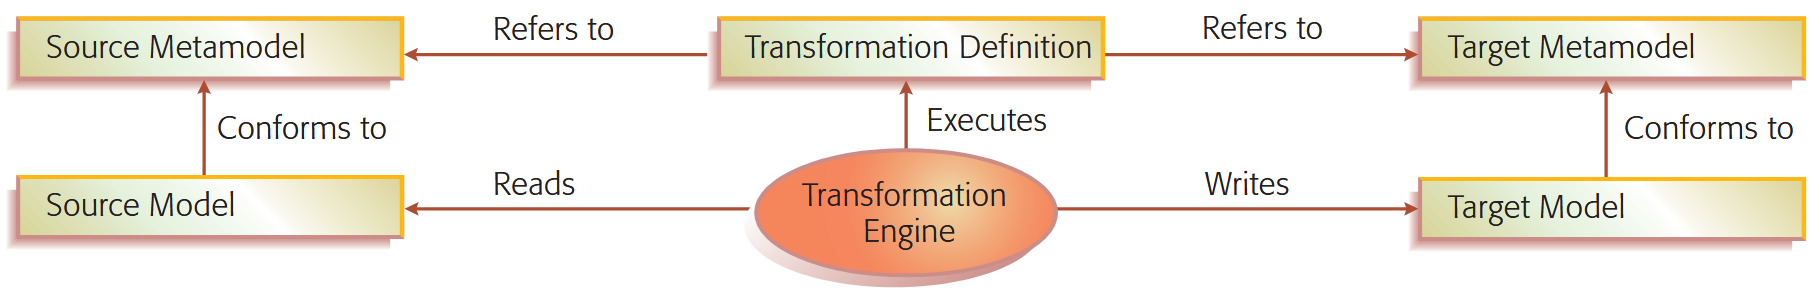
\includegraphics[width=13cm]{figures/model_transformation.png}
\caption{Schematic example of a model transformation with one source and one target model.\cite{czarnecki_helsen_feature_based_survey_2006}}
\label{fig:ModelTransformation}
\end{figure}

Semantic properties often cannot be distinctly related to a single model if a system is composed of multiple models that are developed together; however loosely coupled, a certain \emph{semantic overlap} between these models occurs. Consistency preservation rules (CPRs) in the \textsc{Vitruvius} approach \cite{VitruviusKlare2021} realize some semantic considerations, in that case those concerning consistency, to relations between models, which are realized by model transformations.


\subsection{Model Synchronization}
\label{sec:Foundations:ModelSynchronization}
In order to keep models that have a semantic overlap consistent, a change that occurs in one model has to be propagated to another model if the change concerns the semantic overlap. This synchronization process can be realized with model transformations that have certain features. 
In their model transformation classification approach, Czarnecki and Helsen identify features that can be used to characterize different approaches to consistency preservation. \cite{czarnecki_helsen_feature_based_survey_2006}
The incrementality features are necessary properties for model synchronization, while directionality and tracing classify synchronization transformations.

\paragraph{Incrementality} 
Incrementality comprises the features target incrementality, source incrementality, and preservation of user edits in the target.
\emph{Target incrementality} describes whether a transformation is able to propagate changes in the source model to an existing target model. Since consistency preservation requires propagating consistency-breaking changes in one model to another model with which it semantically overlaps, that is a necessary property of consistency preservation transformations.
A transformation has the feature of \emph{source incrementality} if it \enquote{minimizes the amount of source that needs to be reexamined by a transformation}.
This property is desirable from a performance point of view and with regard to potential information loss.
\emph{Preservation of user edits in the target} describes the ability of a transformation to apply source model changes to the target model while preserving modifications in the target model. A transformation that is target incremental but does not preserve user edits in the target is undesirable for consistency preservation purposes, since it may discard user edits and thus introduce information loss.

\paragraph{Directionality}
If a transformation can be executed in only one direction, it is called \emph{unidirectional}, otherwise it is called \emph{multidirectional}.
A \emph{bidirectional} transformation is a kind of multidirectional transformation that can be executed in two directions.
In the context of model synchronization, where forward and backward transformations are required if both models are subject to user change, bidirectionality of a transformation reduces the definition effort of transformations and ensures that the forward transformation does the same as the backward transformation. If those are separate unidirectional transformations, 
ensuring that they apply the same definition of consistency has to be done elsewise, e.g., by the vigilance of the transformation developer or by deriving the unidirectional transformations from a shared consistency definition, like it is done in the Commonalities Language \cite{klare_commonalities_2019}, which can thus be called bidirectional.

\paragraph{Tracing} is described by Czarnecki and Helsen as a \enquote{runtime footprint of transformation execution}. It is a relevant property for model synchronization transformations since it eases the identification of what model elements have to be changed in the target model.



\section{Single Underlying Models}
Single Underlying Models (SUMs) \cite{atkinson_orthographic_2010_SUM_paper} are an approach to keeping a system consistent by using only one model to represent the system and defining views that are generated via model transformation and are used to access the model.
This kind of approach can be called projective, since views are generated by \enquote{extraction from an underlying repository} \cite{iso_42010}.
This approach has the advantage, that no consistency-keeping has to be done between pairs of models because all information is contained in the SUM.

The benefit of total consistency comes with the drawback of a SUM being monolithic and thus, in larger projects, too complex to be handled by the methodologist responsible for creating the metamodel and view transformations.
Wanting to keep the benefit of consistency while breaking complexity by using multiple metamodels internally, Klare et al. proposed the concept of a \emph{Virtual Single Underlying Metamodel} V-SUMM, with V-SUMs describing the respective instances of the V-SUMM \cite{VitruviusKlare2021}.
A V-SUM internally consists of multiple models but behaves like a SUM to the users who work with the views, since it is also only accessed via views, as shown in \autoref{fig:SUM_vs_VSUM}.
The model instances of these metamodels that share common information have to be kept consistent via model transformations. 

\section{The \textsc{Vitruvius} Approach}
\label{sec:Foundations:Vitruvius}
As an approach to realize a V-SUM, Klare et al. developed the \textsc{Vitruvius} approach \cite{VitruviusKlare2021}.
What exactly is to be kept consistent is abstractly defined by the concept of \emph{consistency preservation rules}, which is reified by the usage of languages like  the Reactions Language and the Commonalities Language.
The \textsc{Vitruvius} approach keeps track of consistency relations by letting CPRs use a correspondence model that helps identify what model elements are to be kept consistent.

\begin{figure}
\centering
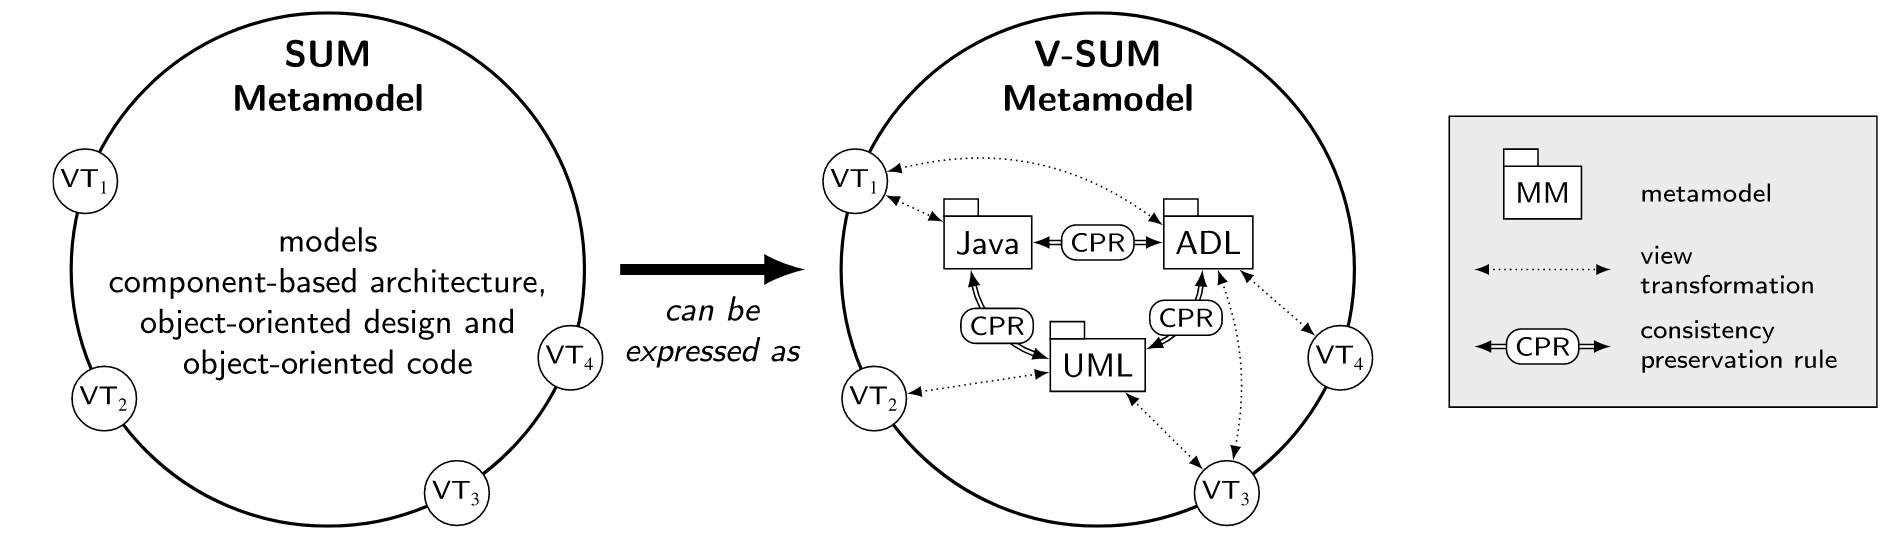
\includegraphics[width=15cm]{figures/SUM_vs_VSUM.png}
\caption{A V-SUM compared to a SUM. From \cite{VitruviusKlare2021}}
\label{fig:SUM_vs_VSUM}
\end{figure}

\subsection{Change Definition}
Changes in \textsc{Vitruvius} are defined via a change metamodel, which itself is defined in Ecore, a meta-metamodel that closely resembles OMG's Essential Meta Object Facility (EMOF), which is supported by the Eclipse Modeling Framework (EMF) as an alternate serialization of Ecore \cite[p. 39]{steinberg_emf_2008}.
Ecore is supported for representing metamodels in \textsc{Vitruvius} \cite{kramer_specification_2017}.

This change metamodel consists of change meta-classes that concern atomic changes and compound changes that group atomic changes, marking that \enquote{these atomic changes occurred together} \cite{kramer_specification_2017}. 
These compound changes are not explicitly modeled in Ecore, however, but are represented in the implementation.

The \textsc{Vitruvius} change metamodel incorporates a class hierarchy with multiple subconcepts of what a change can be.
The root entity is an \emph{EChange}.
Multiple subclasses are additive or subtractive (by inheriting the respective abstract class),
representing adding or deleting something from the model.

There are kinds of changes for 
\begin{itemize}
    \item EObjects: abstract classes for deletion, creation, and existence changing
    \item attribute and reference changes of EObjects: change classes that concern lists, single- or many-valued attributes and references.
    \item root EObjects that are not added by referencing another element
\end{itemize}
To map changes to model entities, the change classes are generically typed with Ecore classes, which represent the model elements to which changes are referring.
As an example, a change to insert a new value into a many-valued attribute is modeled like in \autoref{fig:InsertEAttributeValue}.

\begin{figure}[h]
\centering
\begin{lstlisting}
InsertEAttributeValue<Element extends EJavaObject, 
                      Value extends EJavaObject> 
    -> InsertInListEChange<Element, EAttribute, Value>,
       AdditiveAttributeEChange<Element, Value>
\end{lstlisting}
\caption[\emph{InsertEAttributeValue} signature]{\emph{InsertEAttributeValue} signature. InsertEAttributeValue inherits \emph{InsertInListEchange} and \emph{AdditiveAttributeEChange}}
\label{fig:InsertEAttributeValue}
\end{figure}

\subsection{Correspondence Model}
\label{subsec:Foundations:Vitruvius:CorrespondenceModel}
To trace which elements are to be kept consistent, \textsc{Vitruvius} uses a \emph{correspondence model}. CPRs use that model to trace relations between elements that are to be kept consistent.
This model basically consists of a simple abstract \emph{Correspondence} class that has a tag for storing metadata to \enquote{distinguish different correspondences between the same element} \cite{VitruviusKlare2021} and two fields for left and right objects that are mapped to each other by being part of the same entity, as can be seen in \autoref{fig:VitruviusCorrespondenceModel}.

\begin{figure}[h]
\centering
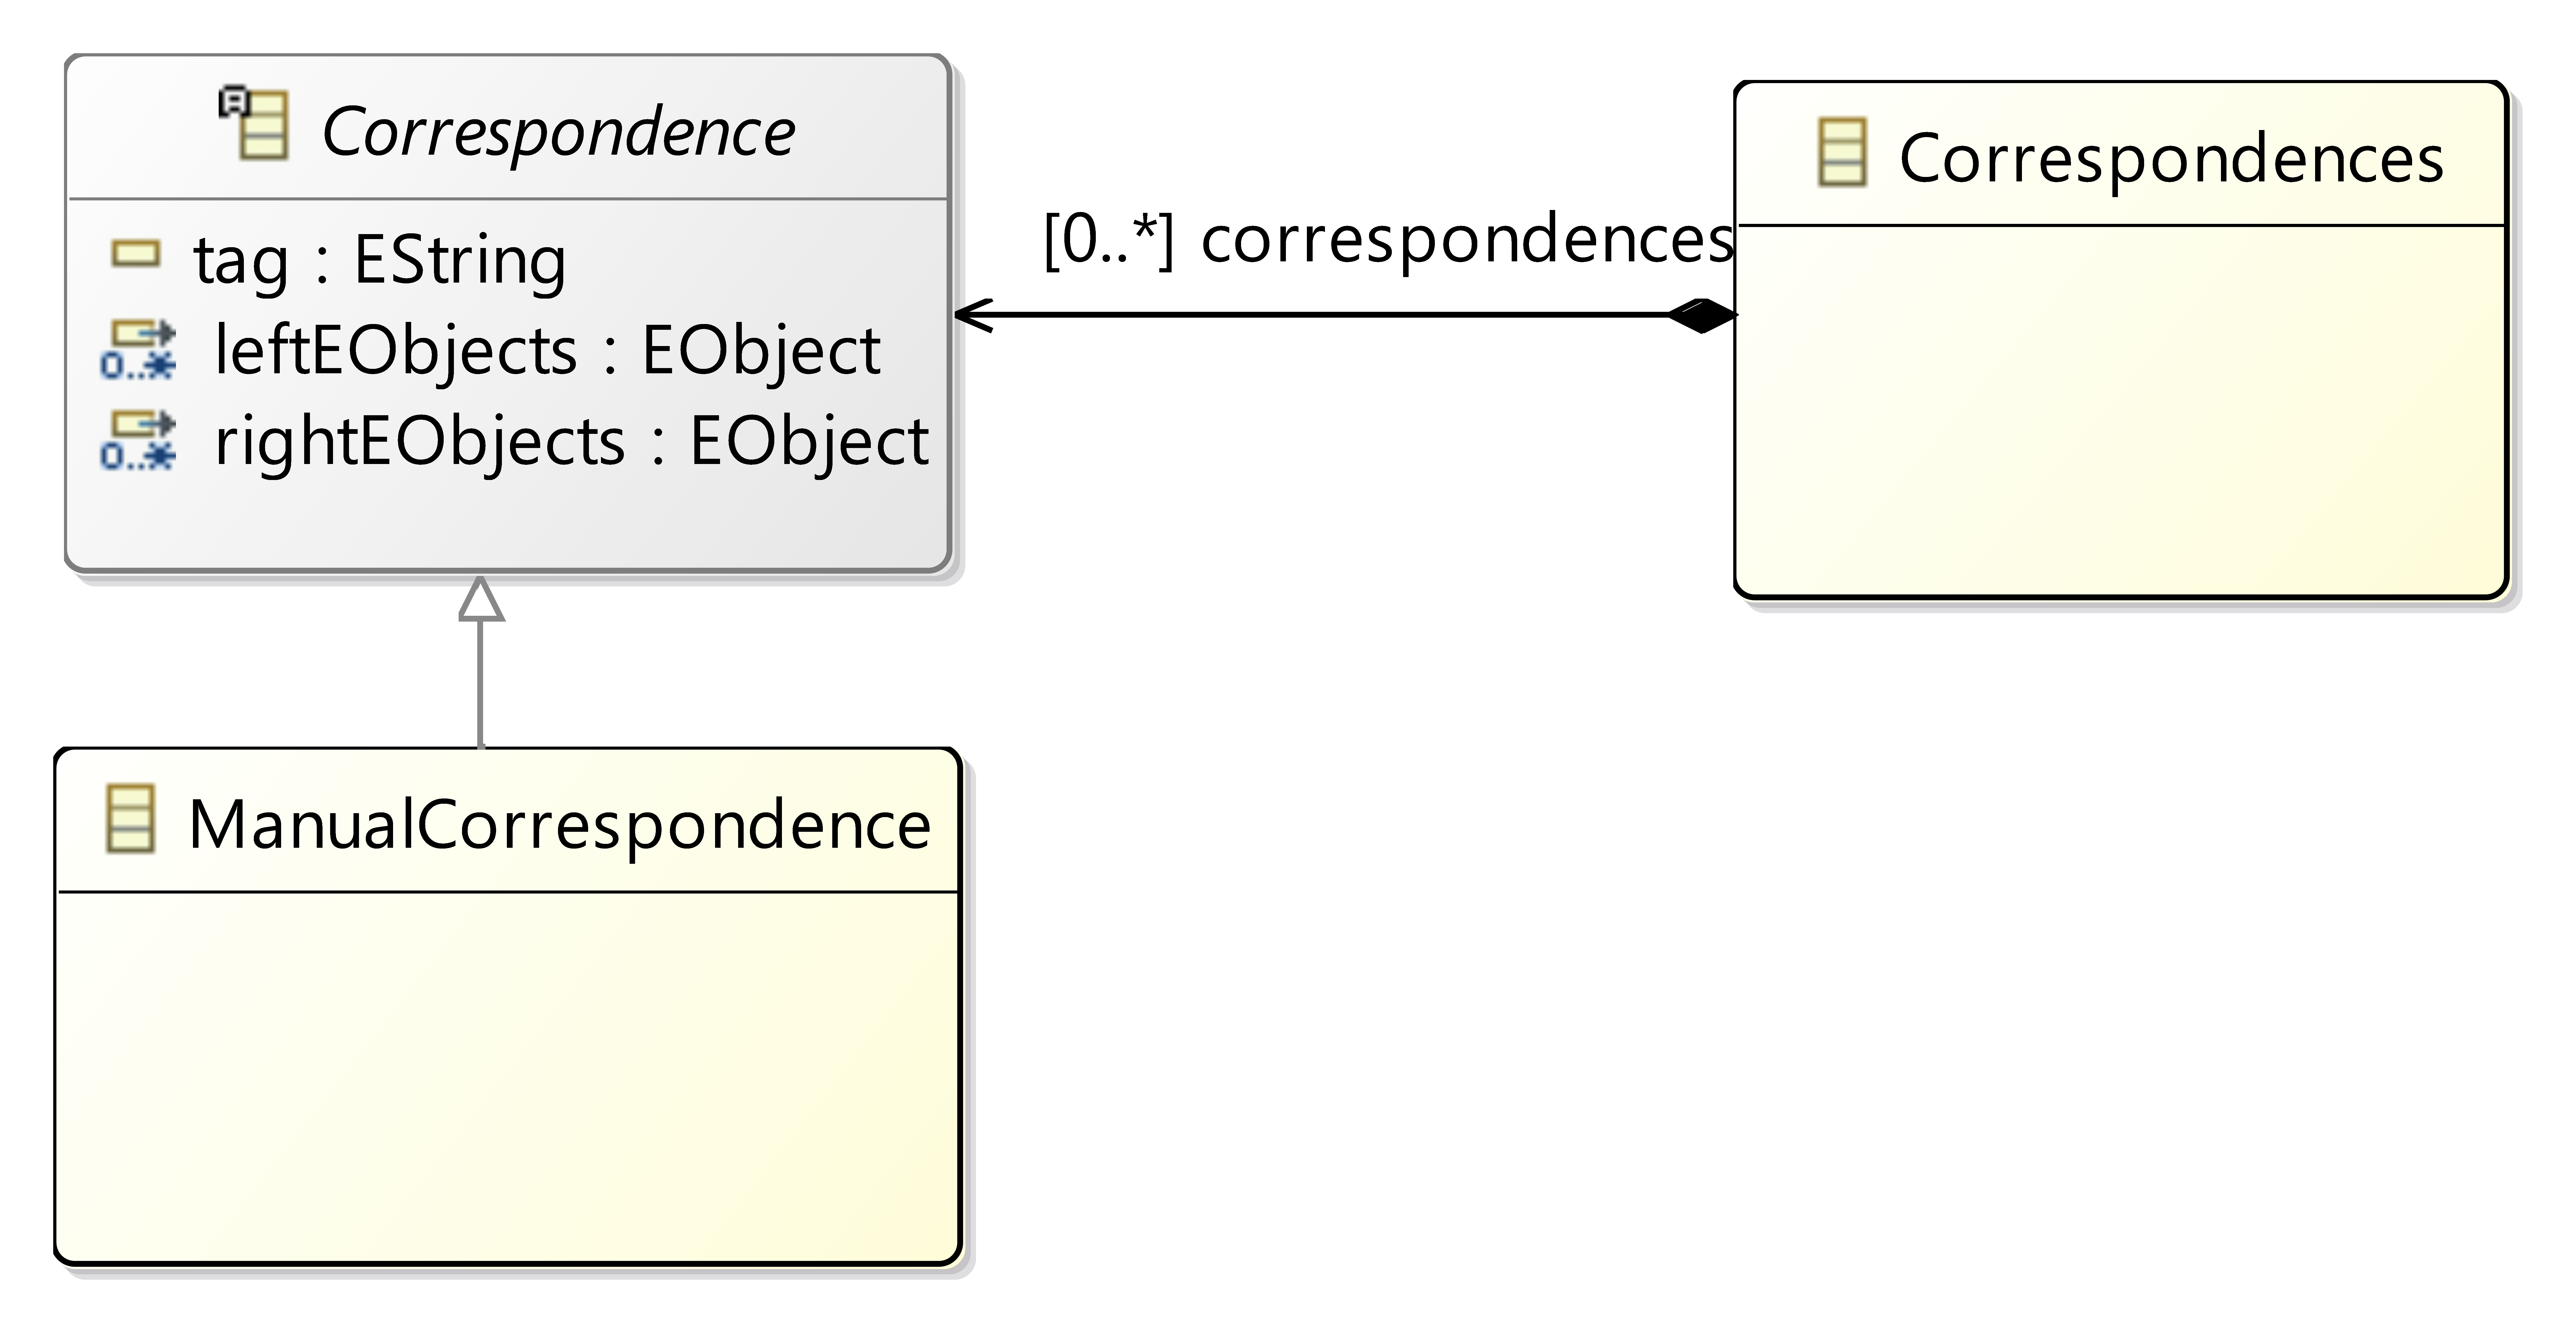
\includegraphics[width=10cm]{figures/vitruvius_correspondence_model.jpg}
\caption{The \textsc{Vitruvius} correspondence model. Generated from the current model definition \cite{vitruvius_correspondence_model_github_ecore}}
\label{fig:VitruviusCorrespondenceModel}
\end{figure}


\section{Triple Graph Grammars} 
\label{sec:Foundations:TGGs}

Schürr\cite{schurr_tggs_1995}, who introduced Triple Graph Grammars, describes them as graph grammars or graph rewriting systems that rewrite three graphs in parallel while explicitly modeling inter-graph relationships in one of the graphs, the \emph{correspondence graph}. 

\paragraph{Graph Grammars} \emph{Graph Grammars} or \enquote{graph rewriting systems} \cite{schurr_tggs_1995} are sets of rules that are semantically similar to productions known from formal language grammars. These rules work in the following way: 
An object diagram, called \emph{left-hand side}, represents a pattern that has to be found in a graph so that the rule can be applied.
The \emph{right-hand side} of the rule represents how that subgraph looks like after transforming the left-hand side via application of the rule.
If all elements on the left-hand side can be identified with an element on the right-hand side, the rule is called a \emph{non-deleting rule}.
In such cases, each element on the left-hand side is identified with an element on the right-hand side; in \autoref{fig:GraphGrammarRuleExample} this is depicted by arrows between the left- and right-hand sides.
For deleting rules, only some elements on the left-hand side can be identified with elements on the right-hand side. To be able to maintain edges between the subgraph that is matched with the left-hand side and the rest of the graph, a \emph{context graph} or \emph{glue graph} is identified that contains the elements that are shared between the left-hand side and the right-hand side and remain unaffected by the transformation \cite{ehrig_introduction_to_graph_grammers_1992}.

\begin{figure}[h]
\centering
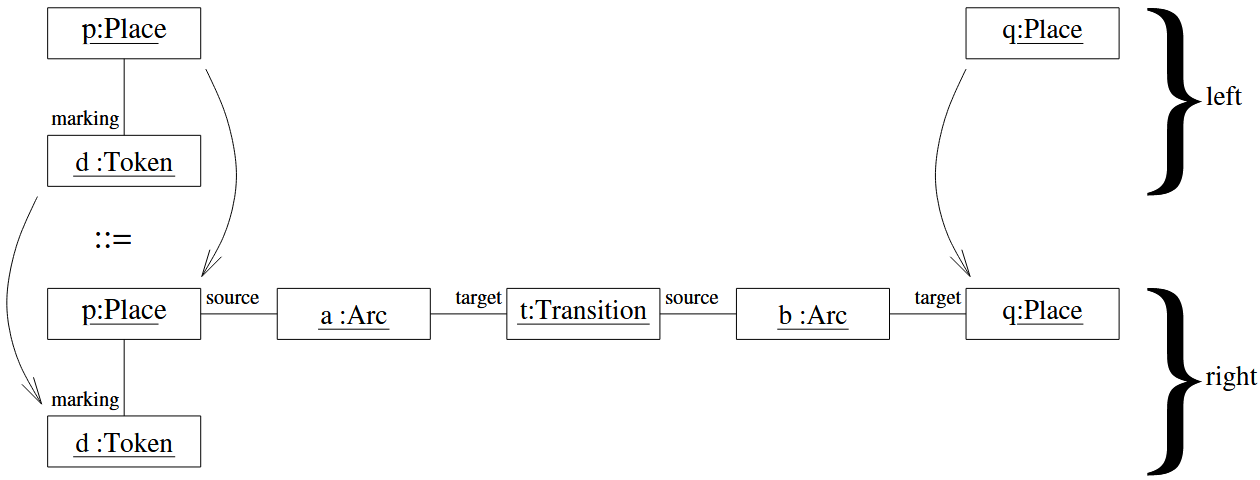
\includegraphics[width=14cm]{figures/graph_grammar_rule_example.png}
\caption{A non-deleting graph grammar rule. \cite{kindler_wagner_triple_graph_grammars_TGG}}
\label{fig:GraphGrammarRuleExample}
\end{figure}

While Graph Grammars are described as \enquote{well-suited for the description of complex transformation or inference processes on complex data structures} \cite{schurr_tggs_1995}, they are limited to specifying in-place modifications within only one graph.

\paragraph{Triple Graph Grammars} \emph{Triple Graph Grammars} (TGGs) were introduced by Schurr \cite{schurr_tggs_1995} to extend this capability to model relationships between two (or more) graphs, thus allowing for simultaneous evolution of models while accounting for their relationship.
This is achieved by an explicitly modeled correspondence graph and a rule set that maps one model triplet, consisting of source, target, and correspondence graph, to another triplet in a similar way, as described for graph grammars in general. The first triplet (left-hand side) again represents the pattern to be found in the graph, which constitutes of the source, target and correspondence graphs. The second triplet (right-hand side) represents that subgraph after transformation.

\paragraph{Model Synchronization with TGGs}
This way, TGG rules also can be used to describe what has to be changed in a target graph when a change in the source graph occurs. If such a change is matchable to the left-hand side and right-hand side of a TGG \emph{source rule}, meaning the part of the TGG rule that concerns the source graph, the respective target rule can be applied to the target graph. The correspondence graph directly references the subgraph in the target graph to which the target rule has to be applied.
That process, from change occurring in the source to applying the matching change in a target graph, represents the application of the TGG rule on the triple graph.
Since the labeling of the source and target graphs as \enquote{source} and \enquote{target} is arbitrary, TGG rules can be described as bidirectional synchronization transformations.

Representing the deletion and modification of elements with TGGs can be done by inversely applying TGG rules, by rolling back rule applications, removing the rule application that created the element one wants to delete, and reapplying rule applications. Both of these approaches can introduce information loss in the target model if a modification is represented. In the inversion case, a modification would be represented as an inverse application of a TGG rule, followed by a re-application of the same rule, but not inversed and with other parameters or another rule. Since the inverse application deletes model elements in the target model that might be enriched with other model elements that are not covered by the TGG rules, information loss can occur. The same problem occurs with the rollback approach.
In certain situations, only inverting a rule application is not sufficient to represent a deleting change, e.g., when two model elements were generated together, in the sense that both creations are represented by one rule application, and later, only one of these is to be deleted. Then, the one that is not to be deleted, hinders the mere application of the inverse rule. In that case, it either would have to be re-created after inversion, or the rollback approach would need to be done. 
So both approaches to handling deleting and modifying changes may introduce information loss in the target model.
Having reviewed different approaches for handling these situations, Fritsche et al. come to the conclusion that an approach that \enquote{avoids unnecessary information loss, is proven to be correct, and is efficiently implemented}, is still missing \cite{fritsche_short-cut-rules-repair-tgg_2021}.
They present \emph{short-cut rules} \cite{fritsche_short-cut-theoretical_2018, fritsche_short-cut-rules-repair-tgg_2021}, which are an approach to cope with the problem of information loss by combining the inverse rule and the other rule. Nodes that would be deleted in the first and re-created in the second rule application are found out and retained in the left-hand sides and right-hand sides of the resulting short-cut rule.
While the original short-cut rules were created at compile time, Fritsche et al. recently presented higher-order short-cut rules \cite{fritsche_higher_order_short_cut_rules_2023} which are generated at runtime to cover more rule combinations and thus further decrease information loss in the target model.
Short-cut rules can be viewed as an effort to improve incrementality features of TGGs for model synchronization, as described in \autoref{sec:Foundations:ModelSynchronization}.
% \subsection{Change Definition}
% \todo{Das unten ist net so ganz das Wahre. --> Beschreiben, was rule patterns sein können und was nicht (z.B. keine Deletes, warum und so...)}

%The change metamodel in TGGs is defined by specifying the set of patterns/ rules of the TGG. \todo{Bild!}
%Thus, it consists of arbitrarily complex left-hand and right-hand side patterns of subgraphs of the involved models plus the correspondence model, which consists of nodes that connect the right-hand and the left-hand side.
%A concrete implementation of such 

\section{eMoflon::IBeX}
\label{sec:Foundations:eMoflon}
eMoflon::IBeX \cite{eMoflonIBeX_weidmann_incremental_nodate} is a tool suite for TGGs which implements model generation, transformation, and synchronization, as well as consistency checking.
It encompasses a strategy to allow for information-preserving model changes in many cases, which is non-trivial and reduces rule-writing overhead. This is done by synthesizing \emph{short-cut rules} \cite{fritsche_short-cut-rules-repair-tgg_2021, fritsche_higher_order_short_cut_rules_2023} that combine one rule that is to be revoked with another rule that replaces it. The resulting rule preserves the entities that would otherwise have been deleted and re-created. Especially if the rule invocation has been done relatively early, this becomes crucial if one does not want to lose information in the deleted-and-recreated entities that is not part of the TGG modeling and can thus not be recreated together with the entities.
% The recreation process is \todo{or can be?} done at runtime \todo{cite 2nd shortcut pepper} so that \dots

Correspondences in eMoflon::IBeX are modeled similarly to, but differently from how \textsc{Vitruvius} \cite{VitruviusKlare2021} models them (see \autoref{subsec:Foundations:Vitruvius:CorrespondenceModel}).
% \todo{Das beschreibt nur, wie man sie definiert, nicht, wie sie intern verwendet werden}
In eMoflon::IBeX, the \emph{schema} defines a correspondence metamodel between two metamodels, whose instances are to be kept consistent.
See \autoref{foundationsEmoflonSchema} for an example schema definition and \autoref{foundationsEmoflonRuleExample} for an example usage of this schema in a rule definition.
This correspondence metamodel is then used in rule definitions to model the actual correspondences between entities of source and target.
The correspondences are modeled similarly to how \textsc{Vitruvius} does it, correspondence types are given a name and source and target EClasses. One noteworthy difference is that in \textsc{Vitruvius}, the user does not pre-define an explicit correspondence metamodel, which is used to manage correspondences in the CPRs, but instantiates the existing correspondence metamodel, which is shown in \autoref{fig:VitruviusCorrespondenceModel}. In the \emph{Reactions} language, described in \autoref{ch:RelatedWork}, this metamodel is part of the language.


\begin{figure}
\centering
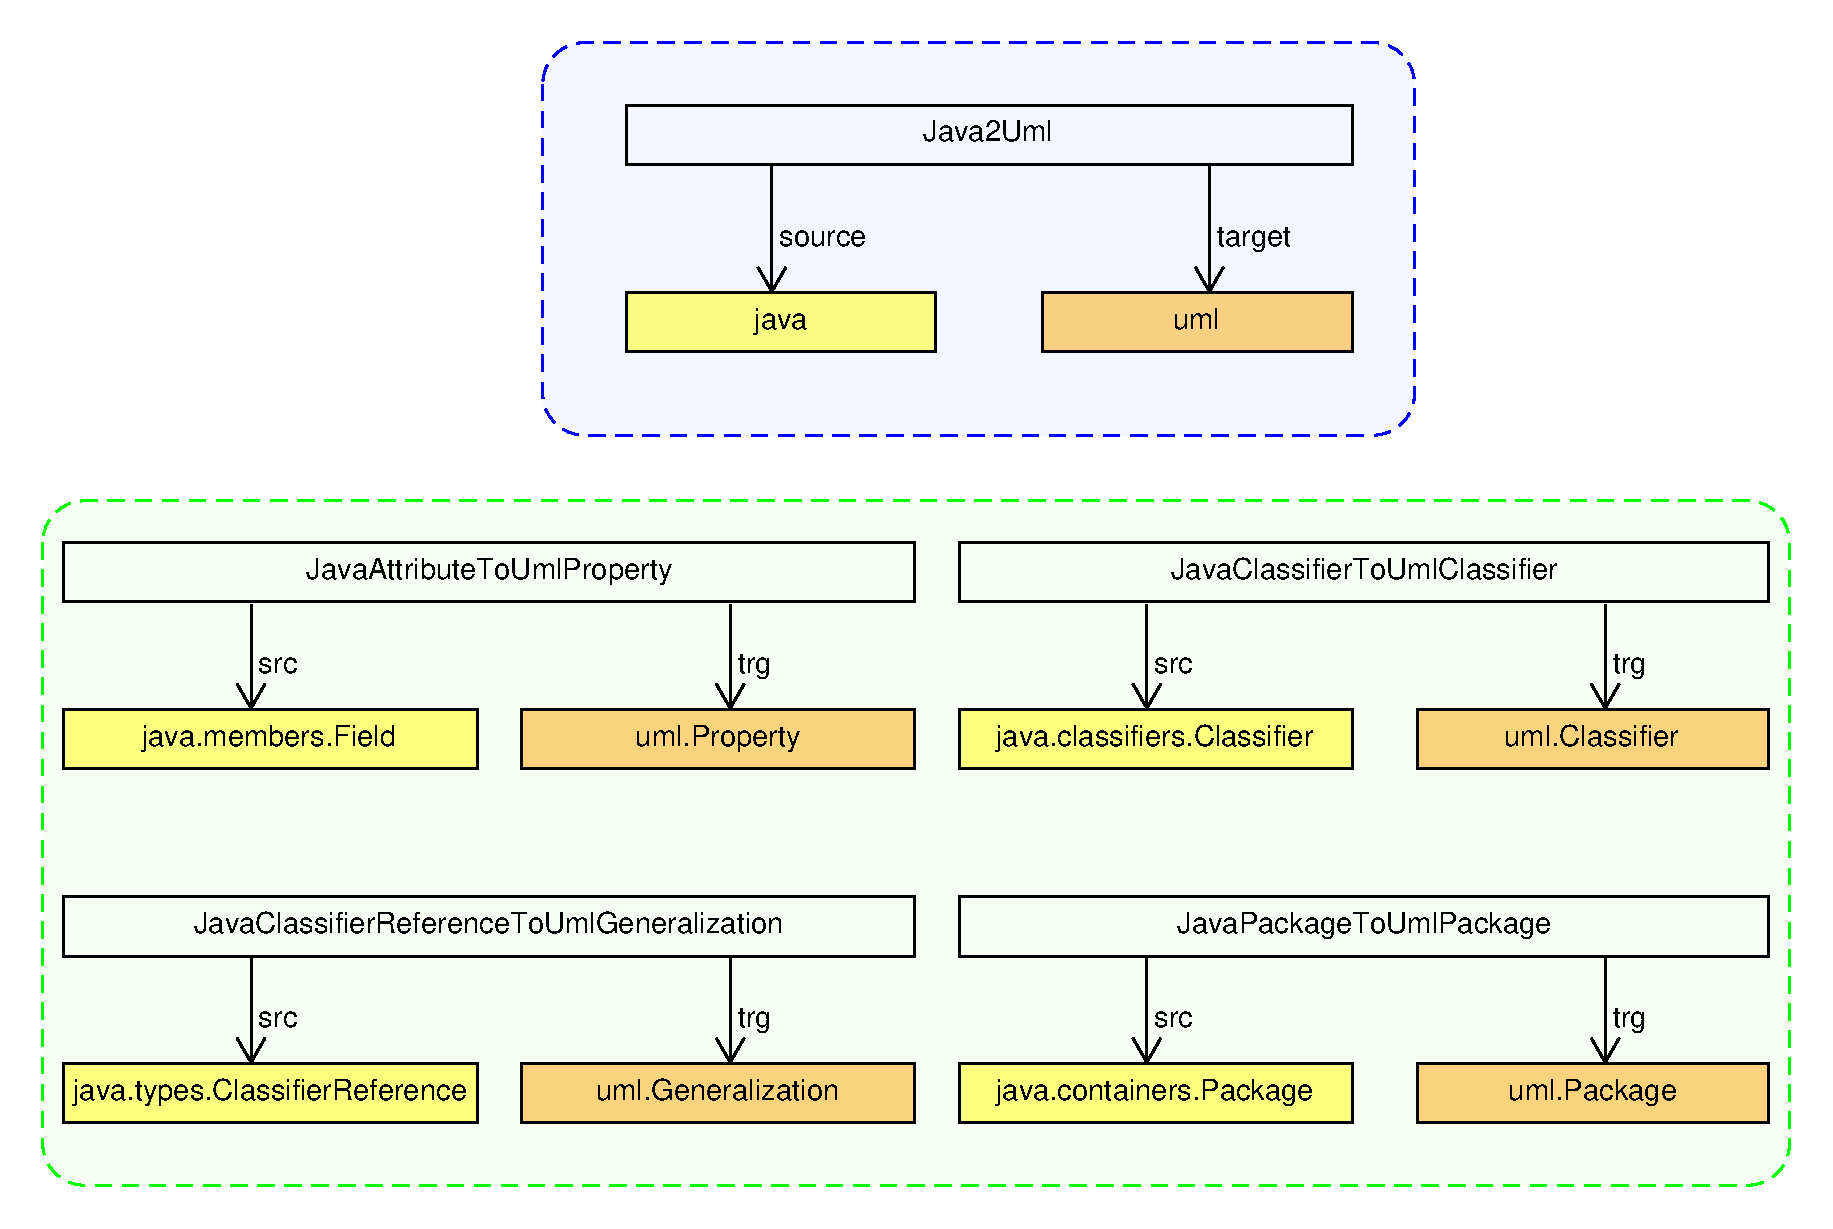
\includegraphics[width=15.5cm]{figures/Java2Uml_schema_excerpt.pdf}
\caption[Schema definition in eMoflon::IBeX]{Schema definition in eMoflon::IBeX: The schema and its source and target metamodel are specified (top), as well as correspondence types (bottom) that refer to EClasses of the respective source and target metamodels.}
\label{foundationsEmoflonSchema}
\end{figure}

\begin{figure}
\centering
% \begin{lstlisting}[language=java, caption={Schema definition in eMoflon::IBeX: Source and target metamodels are defined, as well as correspondence types that refer to EClasses of the respective source and target metamodels.}, captionpos=b, label=foundationsEmoflonSchema]
% #import "platform:/plugin/org.emftext.language.java/metamodel/java.ecore"
% #import "platform:/plugin/org.eclipse.uml2.uml/model/UML.ecore"

% #schema Java2Uml
	
% #source {
% 	java
% }

% #target { 
% 	uml
% } 

% #correspondence {
% 	JavaClassifierToUmlClassifier {
% 		#src->java.classifiers.Classifier
% 		#trg->uml.Classifier
% 	}
% 	JavaPackageToUmlPackage {
% 		#src->java.containers.Package
% 		#trg->uml.Package
% 	}
% 	JavaAttributeToUmlProperty {
% 		#src->java.members.Field
% 		#trg->uml.Property
% 	}
% 	JavaClassifierReferenceToUmlGeneralization {
% 		#src->java.types.ClassifierReference
% 		#trg->uml.Generalization
% 	}
%     ...
% }
% \end{lstlisting}
\end{figure}


\begin{lstlisting}[language=java, caption={Rule defition in eMoflon::IBeX: correspondence relationships can only refer to correspondence classes defined in the \emph{schema} (see \autoref{foundationsEmoflonSchema}). Rules can be abstract and concrete. Inheritance is possible.}, captionpos=b, label=foundationsEmoflonRuleExample]
#using Java2Uml.*
#using AttrCondDefLibrary.*

#abstract #rule AttributeToProperty #with Java2Uml
	#source { 
		classifier:java.classifiers.Classifier
		++field:java.members.Field 
	}
	#target {
		umlClassifier:uml.Classifier
		++property:uml.Property
		
	}
	#correspondence {
		classToUmlClass:JavaClassifierToUmlClassifier {
			#src->classifier
			#trg->umlClassifier
		}
		++attributeToProperty:JavaAttributeToUmlProperty{
			#src->field
			#trg->property
		}
	}
	#attributeConditions { eq_string(field.name, property.name) }

#rule ClassAttributeToProperty #extends AttributeToProperty #with Java2Uml
	#source {
		classifier:java.classifiers.Class {
			++ -members->field
		}
	}
	#target {
		umlClassifier:uml.Class {
			++-ownedAttribute->property
		}
	}
...
\end{lstlisting}




\subsection{Attribute Conditions}
\label{sec:Foundations:eMoflon:attributeConditions}
\emph{Ecore} differentiates between \emph{EObjects} and \emph{EDataTypes}.
Since EDataTypes are not part of the model graph, but fields of EObjects, they cannot be represented in synchronization by plain TGG rules.
To be able to synchronize attributes, \emph{attribute conditions} are used \cite{eMoflonIBeX_weidmann_incremental_nodate, emoflon_tutorial}. 
Attribute conditions define constraints between attributes of the source and target model that must be fulfilled for a TGG rule match to be valid.
In eMoflon::IBeX, the user can define for which attribute states condition checking or enforcement should be applied, and the condition checking/enforcement procedure can depend on that state combination.
An attribute can be in \emph{free} or \emph{bonded} state, depending on whether a value has been assigned to it.
That way, attribute conditions can be used to set free attributes (e.g. in the target model) based on other, bonded attributes (e.g. in the source model), but also to assert a consistency relationship between bonded attributes.
There is a predefined library for common attribute conditions, such as string equality. 
Additionally, custom attribute conditions can be defined by the user.


\subsection{Synchronization Process}
\label{sec:Foundations:eMoflon:syncProcess}
eMoflon::IBeX implements the synchronization process described by Fritsche et al. \cite{fritsche_short-cut-rules-repair-tgg_2021}, which is based on a synchronization algorithm that uses an \emph{incremental pattern matcher} that provides currently applicable and broken TGG rule matches, from which the synchronization chooses what to apply. 
In \autoref{fig:emoflonSynchonizationProcess}, the synchronization process is shown in a simplified version.
By calling the pattern matcher on a possibly unsynchronized triple graph, new TGG rule matches, called \enquote{forward matches}, are calculated, as well as matches that have existed before calling the pattern matcher and have become invalid (\enquote{broken}).
If no forward or broken matches were calculated, the algorithm terminates.
Else, if forward matches are present, one is chosen and applied, and the process is started anew.
If no forward matches are present, but broken matches are, they are attempted to be repaired via short-cut rules (see \autoref{sec:Foundations:TGGs}, \cite{fritsche_short-cut-theoretical_2018, fritsche_short-cut-rules-repair-tgg_2021, fritsche_higher_order_short_cut_rules_2023}).
Remaining broken matches that could not be repaired, are revoked, freeing nodes of the triple graph and possibly enabling new forward matches. Thus, again, the process is started anew, after the revoking step.

\begin{figure}
\centering
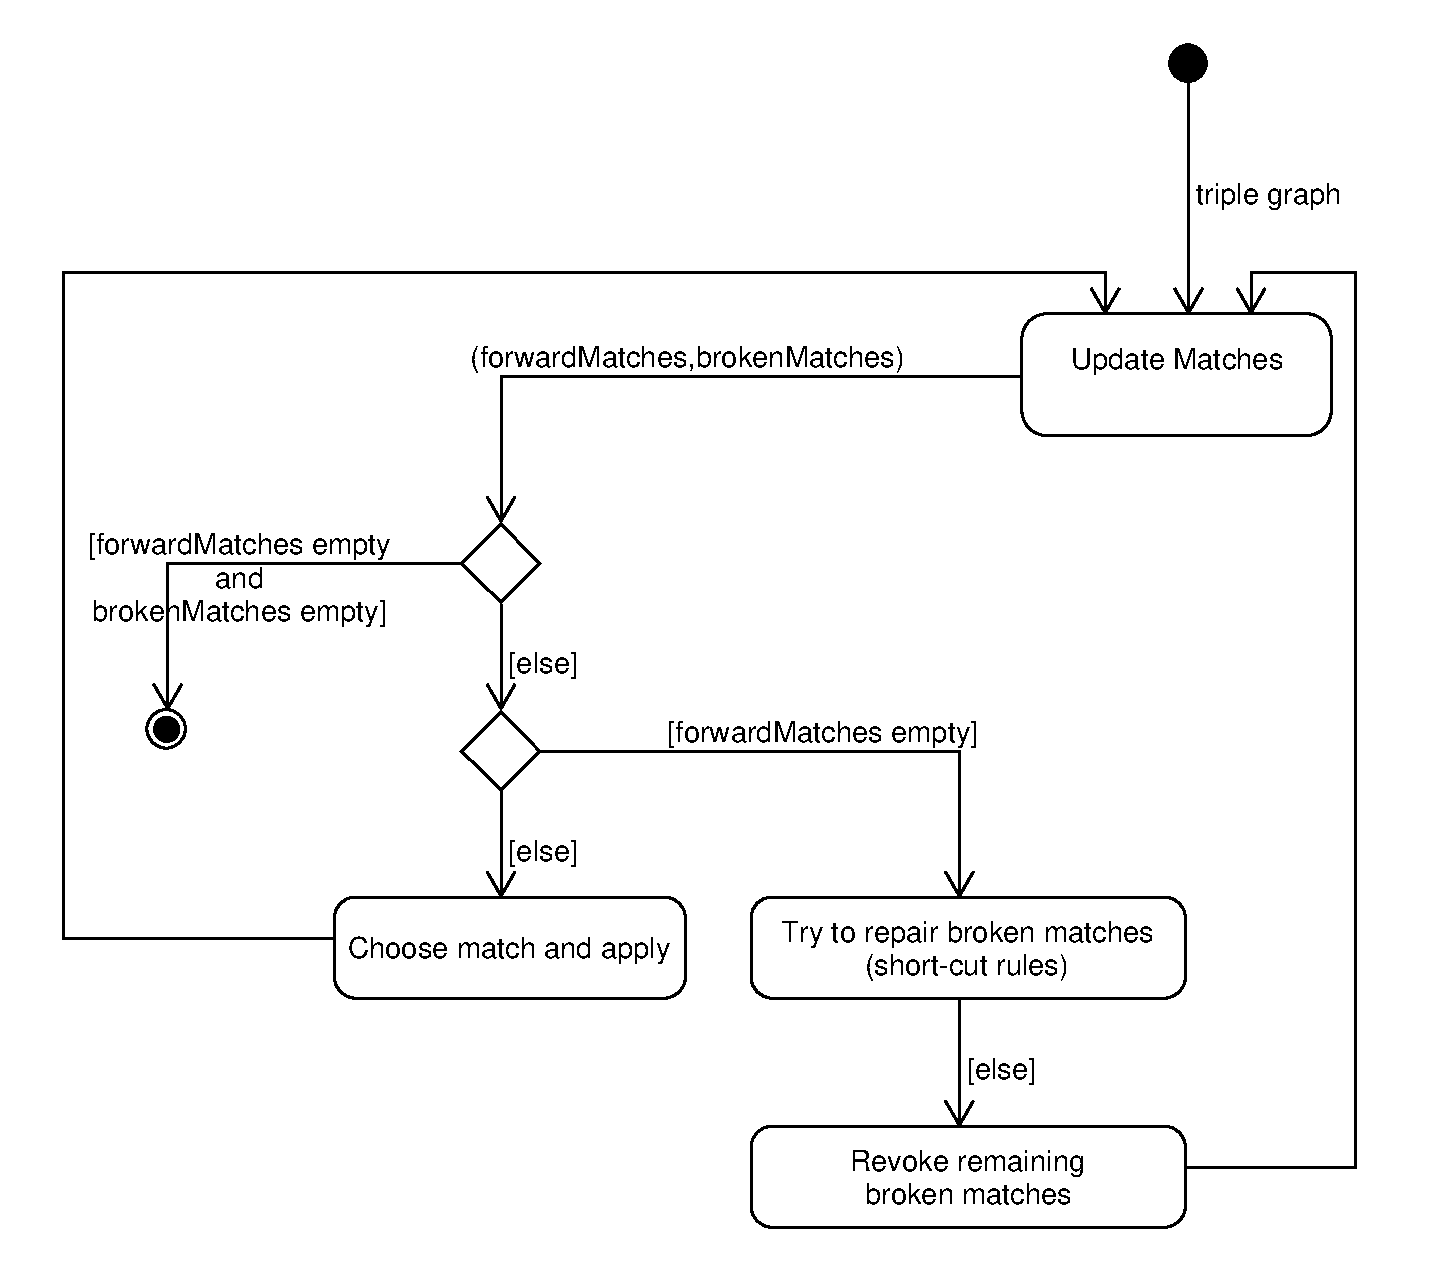
\includegraphics[width=15cm]{figures/emoflonSynchonizationProcess.pdf}
\caption[Activity diagram of the synchronization process in \emph{eMoflon::IBeX}]{Simplified activity diagram based on the synchronization process in \emph{eMoflon::IBeX} based on the synchronization algorithm presented in \cite{fritsche_short-cut-rules-repair-tgg_2021}. Arrow labels in \texttt{[brackets]} indicate control flow, other labels indicate data flow.}
\label{fig:emoflonSynchonizationProcess}
\end{figure}

\section{Detection of Complex Changes}
\label{sec:Foundations:ComplexChangeDetection}
Identifying and choosing complex change patterns in sequences of atomic changes has been researched by Khelladi et al. \cite{khelladi_detecting_complex_changes_2015} in the context of metamodel evolution, aiming to better and more coarsely grained represent the intention of users than with the atomic changes \enquote{add, delete, and update elements}.
To deal with the challenge of complex change patterns overlapping after identifying these patterns in a sequence, they introduce three heuristics, which are briefly explained in the following:

\paragraph{Containment heuristic} For applying the \emph{containment heuristic}, each complex change pattern is assigned a \emph{priority} based on the length of the longest containment path from the pattern under consideration to another pattern it contains. As an example, let $P_1,P_2,P_3$ be three complex change patterns with the containment relation being $P_3 \subset P_2 \subset P_1$. Then, the priorities are as follows: $priority(P_1)=1, priority(P_2)=2,priority(P_3)=3$.
In applying the containment heuristic, complex change patterns with higher priority are preferred over patterns with lower priority.

\paragraph{Distance of a complex change} The distance heuristic is defined as follows: $Distance = \frac{S_{CC}-1}{EP-SP}$. $S_{CC}$ is defined as the size of the complex change, and $EP$ and $SP$ refer to the end position and the start position of the detected complex change in the change sequence. This heuristic is between $0$ and $1$ and measures how widespread a pattern is relative to its size. A detected complex change that occurs in the change sequence \enquote{without interruption} by other changes has a distance of $1$. Higher distances are preferred to lower distances when choosing between overlapping patterns.

\paragraph{Solving overlapping rate} The \emph{solving overlapping rate} heuristic aims to \enquote{minimize the number of overlapping changes} by removing candidates. Thus, the higher the reduction of remaining overlapping changes that is caused by the removal of a complex change from the candidate list, the higher the solving overlapping rate.
Formally, it is defined as $SolvingOverlappingRate = 1 - \frac{N_{LOCC}}{N_{OCC}}$, $N_{LOCC}$ being the number of overlapping changes that would remain if the currently considered complex change were disregarded, and $N_{OCC}$ being the total number of overlapping complex changes.